\section*{Aufgabe 2}
\subsection*{a)}
Denken Sie sich eine kleine Sprache aus.
Definieren Sie deren Vokabular mit einer ANTLR4 lexer grammar und deren Grammatik mit einer ANTLR4 parser grammar.
Erzeugen Sie für einige Beispieltexte mit Hilfe von \textit{org.antlr.v4.gui.TestRig} den Ableitungsbaum (Parse Tree).

\subsection*{a - Lösung}
Dargestellt ist der Lexer einer Sprache, welche die korrekte Kreation einer Java Klasse darstellt.
Erlaubt sind Variablen - also einzelne Buchstaben, sowie Zahlen.
Parameter werden durch Komma getrennt und dürfen eigene neu erzeugte Klassen sein.
\newline
\begin{lstlisting}[label={lst:Aufgabe2a_lexer}, style=ANTLR]
    // CreationLexer.g4
    lexer grammar CreationLexer;

    KEYWORD : 'new' ;

    NAME : [A-Za-z]+ ;
    NUM : [0-9]+ ;

    COMMA : ',' ;

    PAR_OPEN : '(' ;
    PAR_CLOSE : ')' ;

    WS : [ \t\r\n]+ ;

    InvalidChar: . ;
\end{lstlisting}

\newpage

Der dazugehörige Parser:
\begin{lstlisting}[label={lst:Aufgabe2a_parser}, style=ANTLR]
    // CreationParser.g4
    parser grammar CreationParser;
    options { tokenVocab=CreationLexer; }

    start : expr EOF;

    expr : KEYWORD WS NAME PAR_OPEN params PAR_CLOSE ;

    params : (param (COMMA WS? param)*)? ;

    param : (expr | NAME | NUM) ;
\end{lstlisting}
\newline

\begin{figure}[h]
    \centering
    \subfloat[\centering Input: new Object(1, 2)]{{ 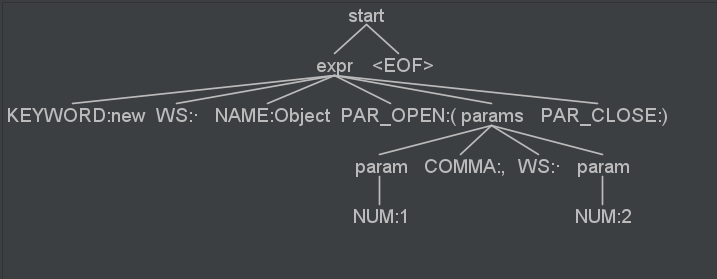
\includegraphics[width=10cm]{images/Aufgabe2a_parseTree_simple} }}
    \qquad
    \subfloat[\centering Input: new Object(1, new Array())]{{ 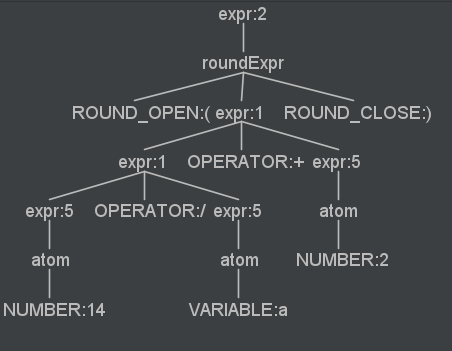
\includegraphics[width=10cm]{images/Aufgabe2a_parseTree} }}
    \caption{Parse Tree Beispiele}
    \label{fig:Aufgabe2a_parseTree}
\end{figure}
\newline

\textbf{Der Parser ist für die grammatikalische Anordnung der durch den Lexer vorgegebenen Token verantwortlich.}
\newpage

\subsection*{b)}
Definieren Sie mit Java-Klassen die abstrakte Syntax Ihrer Sprache aus a) und
schreiben Sie ein Java-Programm, das den ANTLR4 Parse Tree in einen AST überführt.

\subsection*{b - Lösung}
Definition als UML-Diagramm:
\begin{figure}[h]
    \centering
    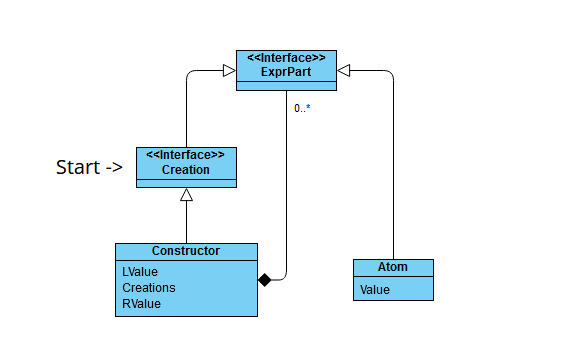
\includegraphics[width=10cm]{images/Aufgabe2b_Diagramm}
    \caption{UML-Diagramm}
    \label{fig:Aufgabe2b_UML}
\end{figure}
\newline
Eine Baumstufe kann in drei Teile geteilt werden:
\begin{itemize}
    \item \textbf{Links}: Der Keyword-, Namen- und Klammer-Teil vor der Mitte.
    \item \textbf{Mitte}: Rekursive Parameter-Definition - kann auch leer oder eine neue \textit{Creation} sein.
    \item \textbf{Rechts}: In diesem Fall die Klammer zum Schließen der Parameter.
\end{itemize}
\newline
Dadurch ergibt sich die Vorgabe von mindestens einer Constructor Instanz.
\textit{L-} und \textit{RValue} sind definierbare Strings und \textit{Creations}
ist die Liste der Parameter innerhalb der Klammern/Strings, dargestellt in der Relation.
So können neue \textit{Constructor} Objekte, sowie Werte definiert in der Klasse \textit{Atom} als Parameter übergeben werden.

\newpage
Um die Struktur beizubehalten, werden beispielhaft also folgende Klassen erstellt:
\begin{lstlisting}[label={lst:Aufgabe2b_Classes}]
public interface Expr {
}

public interface Creation extends Expr {
}

public class Atom implements Expr {
    private final String val;

    public Atom(String val) {
        this.val = val;
    }
    public String getVal() {
        return val;
    }
    @Override
    public String toString() {
        return this.val;
    }
}

public class Constructor implements Creation {
    private final String leftVal;
    private final List<Expr> params;
    private final String rightVal;

    public Constructor(String leftVal, List<Expr> params, String rightVal) {
        this.leftVal = leftVal;
        this.params = params;
        this.rightVal = rightVal;
    }
    public String getLeftVal() {
        return leftVal;
    }
    public List<Expr> getParams() {
        return params;
    }
    public String getRightVal() {
        return rightVal;
    }
    @Override
    public String toString() {
        return this.leftVal + this.params + this.rightVal;
    }
}
\end{lstlisting}

Um diese Struktur in einem Builder umzusetzen, muss ein eigener Stack für
jedes neue Constructor Objekt angelegt werden.

\begin{lstlisting}[label={lst:Aufgabe2b_Builder}]
public class CreationBuilder extends CreationParserBaseListener {

    private final List<Stack<Expr>> stackList = new LinkedList<>();
    private int depth = -1;

    public Creation build(ParseTree tree) {
        new ParseTreeWalker().walk(this, tree);

        return (Creation) this.stackList.get(this.depth).pop();
    }

    @Override
    public void enterExpr(CreationParser.ExprContext ctx) {
        this.stackList.add(new Stack<>());
        this.depth++;
    }

    @Override
    public void exitExpr(CreationParser.ExprContext ctx) {
        if (ctx.getChildCount() == 6) {
            var l = new StringBuilder();
            for (int i = 0; i < 4; i++) {
                l.append(ctx.getChild(i).getText());
            }


            var c = new Constructor(
                    l.toString(),
                    new LinkedList<>(this.stackList.get(this.depth)),
                    ctx.getChild(5).getText()
            );
            this.stackList.get(this.depth).clear();

            if (this.depth > 0)
                this.depth--;
            this.stackList.get(this.depth).push(c);

        }
    }

    @Override
    public void enterParam(CreationParser.ParamContext ctx) {
        if (ctx.start.getType() == CreationParser.NUM) {

            this.stackList.get(this.depth).push(new Atom(ctx.NUM().getText()));

        } else if (ctx.start.getType() == CreationParser.NAME) {

            this.stackList.get(this.depth).push(new Atom(ctx.NAME().getText()));

        }
    }

}
\end{lstlisting}

Für jedes angefangene Constructor Objekt wird ein neuer Stack angelegt in der \textit{enterExpr} Methode.
Zusätzlich wird die Tiefe erhöht, um jeweils beim aktuell noch nicht abgeschlossenen Constructor Objekt zu bleiben.
Dadurch bleibt die Reihenfolge erhalten und innerhalb eines noch nicht abgeschlossenen Constructor Objekts können
\textit{Atom} Objekte und weitere \textit{Constructor} Objekte erstellt werden, ohne dass Konstruktoren die
auf dem Stack liegenden Objekte in sich aufnehmen.
\newline
\newline
Die \textit{exitExpr} Methode arbeitet den aktuellen Stack ab und setzt ihn als Parameter-Liste für das
aktuelle \textit{Constructor} Objekt.
Danach wird der aktuelle Stack geleert und die Tiefe verringert.
Abschließend wird der aktuelle Konstruktor auf den Stack gelegt für den nächsten Konstruktor oder
den finalen Rückgabewert.
\newline
\newline
Die \textit{enterParam} Methode ist der unterste Baustein des Baums,
und dient zur Erstellung von \textit{Atom} Objekten, die dann auf den Stack gelegt werden für Konstruktoren.
Wenn die \textit{Param} Regel wieder eine \textit{Expr} Regel enthält, wird sie in der Methode ignoriert,
da diese bereits in der \textit{exitExpr} Methode abgearbeitet wird.

\newpage